\documentclass[border=4pt]{standalone}

\usepackage{amsmath}
\usepackage{tikz}
\usepackage{mathdots}
\usepackage{yhmath}
\usepackage{cancel}
\usepackage{color}
\usepackage{siunitx}
\usepackage{array}
\usepackage{multirow}
\usepackage{amssymb}
\usepackage{gensymb}
\usepackage{tabularx}
\usepackage{booktabs}
\usetikzlibrary{fadings}
\usetikzlibrary{patterns}


\begin{document}
 
     

\tikzset{every picture/.style={line width=0.75pt}} %set default line width to 0.75pt        

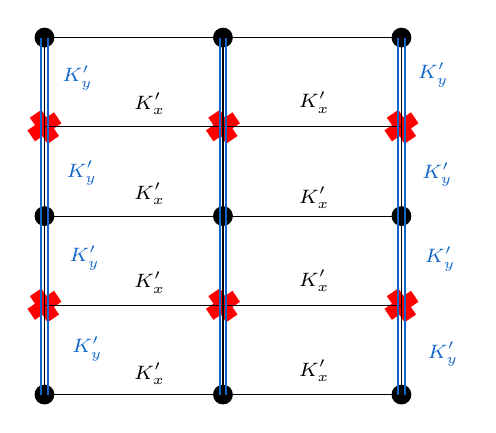
\begin{tikzpicture}[x=0.75pt,y=0.75pt,yscale=-1,xscale=1]
%uncomment if require: \path (0,300); %set diagram left start at 0, and has height of 300

%Shape: Circle [id:dp683429810696621] 
\draw  [color={rgb, 255:red, 0; green, 0; blue, 0 }  ,draw opacity=1 ][fill={rgb, 255:red, 0; green, 0; blue, 0 }  ,fill opacity=1 ] (145.5,65) .. controls (145.5,62.51) and (147.51,60.5) .. (150,60.5) .. controls (152.49,60.5) and (154.5,62.51) .. (154.5,65) .. controls (154.5,67.49) and (152.49,69.5) .. (150,69.5) .. controls (147.51,69.5) and (145.5,67.49) .. (145.5,65) -- cycle ;
%Shape: Circle [id:dp24371107397152825] 
\draw  [color={rgb, 255:red, 0; green, 0; blue, 0 }  ,draw opacity=1 ][fill={rgb, 255:red, 0; green, 0; blue, 0 }  ,fill opacity=1 ] (145.5,151) .. controls (145.5,148.51) and (147.51,146.5) .. (150,146.5) .. controls (152.49,146.5) and (154.5,148.51) .. (154.5,151) .. controls (154.5,153.49) and (152.49,155.5) .. (150,155.5) .. controls (147.51,155.5) and (145.5,153.49) .. (145.5,151) -- cycle ;
%Shape: Circle [id:dp9413426668415599] 
\draw  [color={rgb, 255:red, 0; green, 0; blue, 0 }  ,draw opacity=1 ][fill={rgb, 255:red, 0; green, 0; blue, 0 }  ,fill opacity=1 ] (145.5,237) .. controls (145.5,234.51) and (147.51,232.5) .. (150,232.5) .. controls (152.49,232.5) and (154.5,234.51) .. (154.5,237) .. controls (154.5,239.49) and (152.49,241.5) .. (150,241.5) .. controls (147.51,241.5) and (145.5,239.49) .. (145.5,237) -- cycle ;
%Shape: Circle [id:dp6002437133111644] 
\draw  [color={rgb, 255:red, 0; green, 0; blue, 0 }  ,draw opacity=1 ][fill={rgb, 255:red, 0; green, 0; blue, 0 }  ,fill opacity=1 ] (231.5,237) .. controls (231.5,234.51) and (233.51,232.5) .. (236,232.5) .. controls (238.49,232.5) and (240.5,234.51) .. (240.5,237) .. controls (240.5,239.49) and (238.49,241.5) .. (236,241.5) .. controls (233.51,241.5) and (231.5,239.49) .. (231.5,237) -- cycle ;
%Shape: Circle [id:dp07727484568258047] 
\draw  [color={rgb, 255:red, 0; green, 0; blue, 0 }  ,draw opacity=1 ][fill={rgb, 255:red, 0; green, 0; blue, 0 }  ,fill opacity=1 ] (231.5,151) .. controls (231.5,148.51) and (233.51,146.5) .. (236,146.5) .. controls (238.49,146.5) and (240.5,148.51) .. (240.5,151) .. controls (240.5,153.49) and (238.49,155.5) .. (236,155.5) .. controls (233.51,155.5) and (231.5,153.49) .. (231.5,151) -- cycle ;
%Shape: Circle [id:dp8016240071577909] 
\draw  [color={rgb, 255:red, 0; green, 0; blue, 0 }  ,draw opacity=1 ][fill={rgb, 255:red, 0; green, 0; blue, 0 }  ,fill opacity=1 ] (231.5,65) .. controls (231.5,62.51) and (233.51,60.5) .. (236,60.5) .. controls (238.49,60.5) and (240.5,62.51) .. (240.5,65) .. controls (240.5,67.49) and (238.49,69.5) .. (236,69.5) .. controls (233.51,69.5) and (231.5,67.49) .. (231.5,65) -- cycle ;
%Shape: Cross [id:dp7694734218110462] 
\draw  [color={rgb, 255:red, 255; green, 0; blue, 0 }  ,draw opacity=1 ][fill={rgb, 255:red, 255; green, 0; blue, 0 }  ,fill opacity=1 ] (154.53,101.38) -- (157.82,106.24) -- (154.18,108.71) -- (156.65,112.35) -- (151.58,115.79) -- (149.11,112.15) -- (145.47,114.62) -- (142.18,109.76) -- (145.82,107.29) -- (143.35,103.65) -- (148.42,100.21) -- (150.89,103.85) -- cycle ;
%Shape: Cross [id:dp07009195142465119] 
\draw  [color={rgb, 255:red, 255; green, 0; blue, 0 }  ,draw opacity=1 ][fill={rgb, 255:red, 255; green, 0; blue, 0 }  ,fill opacity=1 ] (326.53,101.38) -- (329.82,106.24) -- (326.18,108.71) -- (328.65,112.35) -- (323.58,115.79) -- (321.11,112.15) -- (317.47,114.62) -- (314.18,109.76) -- (317.82,107.29) -- (315.35,103.65) -- (320.42,100.21) -- (322.89,103.85) -- cycle ;
%Shape: Cross [id:dp5145576679898121] 
\draw  [color={rgb, 255:red, 255; green, 0; blue, 0 }  ,draw opacity=1 ][fill={rgb, 255:red, 255; green, 0; blue, 0 }  ,fill opacity=1 ] (154.53,187.38) -- (157.82,192.24) -- (154.18,194.71) -- (156.65,198.35) -- (151.58,201.79) -- (149.11,198.15) -- (145.47,200.62) -- (142.18,195.76) -- (145.82,193.29) -- (143.35,189.65) -- (148.42,186.21) -- (150.89,189.85) -- cycle ;
%Shape: Cross [id:dp2311714951651005] 
\draw  [color={rgb, 255:red, 255; green, 0; blue, 0 }  ,draw opacity=1 ][fill={rgb, 255:red, 255; green, 0; blue, 0 }  ,fill opacity=1 ] (240.53,101.38) -- (243.82,106.24) -- (240.18,108.71) -- (242.65,112.35) -- (237.58,115.79) -- (235.11,112.15) -- (231.47,114.62) -- (228.18,109.76) -- (231.82,107.29) -- (229.35,103.65) -- (234.42,100.21) -- (236.89,103.85) -- cycle ;
%Shape: Cross [id:dp37380190729131524] 
\draw  [color={rgb, 255:red, 255; green, 0; blue, 0 }  ,draw opacity=1 ][fill={rgb, 255:red, 255; green, 0; blue, 0 }  ,fill opacity=1 ] (240.53,187.38) -- (243.82,192.24) -- (240.18,194.71) -- (242.65,198.35) -- (237.58,201.79) -- (235.11,198.15) -- (231.47,200.62) -- (228.18,195.76) -- (231.82,193.29) -- (229.35,189.65) -- (234.42,186.21) -- (236.89,189.85) -- cycle ;
%Shape: Cross [id:dp39973070773794284] 
\draw  [color={rgb, 255:red, 255; green, 0; blue, 0 }  ,draw opacity=1 ][fill={rgb, 255:red, 255; green, 0; blue, 0 }  ,fill opacity=1 ] (326.53,187.38) -- (329.82,192.24) -- (326.18,194.71) -- (328.65,198.35) -- (323.58,201.79) -- (321.11,198.15) -- (317.47,200.62) -- (314.18,195.76) -- (317.82,193.29) -- (315.35,189.65) -- (320.42,186.21) -- (322.89,189.85) -- cycle ;
%Shape: Circle [id:dp3336404394147878] 
\draw  [color={rgb, 255:red, 0; green, 0; blue, 0 }  ,draw opacity=1 ][fill={rgb, 255:red, 0; green, 0; blue, 0 }  ,fill opacity=1 ] (317.5,65) .. controls (317.5,62.51) and (319.51,60.5) .. (322,60.5) .. controls (324.49,60.5) and (326.5,62.51) .. (326.5,65) .. controls (326.5,67.49) and (324.49,69.5) .. (322,69.5) .. controls (319.51,69.5) and (317.5,67.49) .. (317.5,65) -- cycle ;
%Shape: Circle [id:dp4223611533088747] 
\draw  [color={rgb, 255:red, 0; green, 0; blue, 0 }  ,draw opacity=1 ][fill={rgb, 255:red, 0; green, 0; blue, 0 }  ,fill opacity=1 ] (317.5,151) .. controls (317.5,148.51) and (319.51,146.5) .. (322,146.5) .. controls (324.49,146.5) and (326.5,148.51) .. (326.5,151) .. controls (326.5,153.49) and (324.49,155.5) .. (322,155.5) .. controls (319.51,155.5) and (317.5,153.49) .. (317.5,151) -- cycle ;
%Shape: Circle [id:dp49869076582960226] 
\draw  [color={rgb, 255:red, 0; green, 0; blue, 0 }  ,draw opacity=1 ][fill={rgb, 255:red, 0; green, 0; blue, 0 }  ,fill opacity=1 ] (317.5,237) .. controls (317.5,234.51) and (319.51,232.5) .. (322,232.5) .. controls (324.49,232.5) and (326.5,234.51) .. (326.5,237) .. controls (326.5,239.49) and (324.49,241.5) .. (322,241.5) .. controls (319.51,241.5) and (317.5,239.49) .. (317.5,237) -- cycle ;
%Straight Lines [id:da2952669853328824] 
\draw    (150,65) -- (322,65) ;


%Straight Lines [id:da4653525256364075] 
\draw    (150,237) -- (322,237) ;


%Straight Lines [id:da4955989672254131] 
\draw    (150,194) -- (322,194) ;


%Straight Lines [id:da9380519517510622] 
\draw    (150,151) -- (322,151) ;


%Straight Lines [id:da46901143544970636] 
\draw    (150,108) -- (322,108) ;


%Straight Lines [id:da3365684233907793] 
\draw    (150,237) -- (150,65) ;


%Straight Lines [id:da5311186236308278] 
\draw    (236,237) -- (236,65) ;


%Straight Lines [id:da22325164010574716] 
\draw    (322,237) -- (322,65) ;


%Straight Lines [id:da2964523175174014] 
\draw [color={rgb, 255:red, 18; green, 102; blue, 202 }  ,draw opacity=1 ][line width=0.75]    (323.5,65) -- (323.5,237)(320.5,65) -- (320.5,237) ;


%Straight Lines [id:da08175319332819941] 
\draw [color={rgb, 255:red, 18; green, 102; blue, 202 }  ,draw opacity=1 ][line width=0.75]    (237.5,65) -- (237.5,237)(234.5,65) -- (234.5,237) ;


%Straight Lines [id:da8944364389736847] 
\draw [color={rgb, 255:red, 18; green, 102; blue, 202 }  ,draw opacity=1 ][line width=0.75]    (151.5,65) -- (151.5,237)(148.5,65) -- (148.5,237) ;



% Text Node
\draw (200.67,140.33) node  [font=\scriptsize]  {$K'_{x}$};
% Text Node
\draw (200.67,97) node  [font=\scriptsize]  {$K'_{x}$};
% Text Node
\draw (200.67,183) node  [font=\scriptsize]  {$K'_{x}$};
% Text Node
\draw (200.67,227) node  [font=\scriptsize]  {$K'_{x}$};
% Text Node
\draw (280,225.67) node  [font=\scriptsize]  {$K'_{x}$};
% Text Node
\draw (280,182.33) node  [font=\scriptsize]  {$K'_{x}$};
% Text Node
\draw (280,142.33) node  [font=\scriptsize]  {$K'_{x}$};
% Text Node
\draw (280,96.33) node  [font=\scriptsize]  {$K'_{x}$};
% Text Node
\draw (166,84.33) node  [font=\scriptsize,color={rgb, 255:red, 18; green, 102; blue, 202 }  ,opacity=1 ]  {$K'_{y}$};
% Text Node
\draw (168,130.33) node  [font=\scriptsize,color={rgb, 255:red, 18; green, 102; blue, 202 }  ,opacity=1 ]  {$K'_{y}$};
% Text Node
\draw (169.33,171) node  [font=\scriptsize,color={rgb, 255:red, 18; green, 102; blue, 202 }  ,opacity=1 ]  {$K'_{y}$};
% Text Node
\draw (170.67,215) node  [font=\scriptsize,color={rgb, 255:red, 18; green, 102; blue, 202 }  ,opacity=1 ]  {$K'_{y}$};
% Text Node
\draw (337.33,83) node  [font=\scriptsize,color={rgb, 255:red, 18; green, 102; blue, 202 }  ,opacity=1 ]  {$K'_{y}$};
% Text Node
\draw (339.33,131) node  [font=\scriptsize,color={rgb, 255:red, 18; green, 102; blue, 202 }  ,opacity=1 ]  {$K'_{y}$};
% Text Node
\draw (340.67,171.67) node  [font=\scriptsize,color={rgb, 255:red, 18; green, 102; blue, 202 }  ,opacity=1 ]  {$K'_{y}$};
% Text Node
\draw (342,217.67) node  [font=\scriptsize,color={rgb, 255:red, 18; green, 102; blue, 202 }  ,opacity=1 ]  {$K'_{y}$};


\end{tikzpicture}
\end{document}
